\section{Vocabulaire}

\begin{definition}~
  \begin{itemize}
    \item Une \emph{expérience aléatoire} est une expérience faisant intervenir le hasard, et comportant plusieurs issues (pouvant donner plusieurs résultat). On ne connaît pas, à priori, le résultat d'une telle expérience.
    \item Une \emph{issue} est un résultat possible de l'expérience aléatoire.
    \item L'\emph{univers} est l'ensemble de toutes les issues. Il est généralement noté $\Omega$.
    \item Un \emph{évènement} est un ensemble d'issues.
    \item Un \emph{évènement élémentaire} est un évènement ne comportant qu'une seule issue.
  \end{itemize}
\end{definition}

\begin{exemple}~
  \begin{itemize}
    \item Lancer un dé équilibré à 6 faces et regarder le nombre obtenu est une expérience aléatoire. \og{}Obtenir 2\fg{} et \og{}Obtenir 1\fg{} sont des issues. \og{}Obtenir un nombre pair\fg{} est un évènement.
    \item Choisir un élève au hasard dans la classe est une expérience aléatoire. \og{}Obtenir l'élève X\fg{} est une issue. \og{}Obtenir un garçon\fg{}, \og{}Obtenir une personne aux cheuveux longs\fg{}, \og{}Obtenir un mineur\fg{} sont des évènements.
  \end{itemize}
\end{exemple}

\begin{remarque}
  Dans toute la suite du cours, les univers considérés seront finis.
\end{remarque}

\section{Probabilité}

\begin{definition} On considère une expérience aléatoire.
  \begin{itemize}
    \item La probabilité d'un événement élémentaire est un nombre compris entre 0 et 1, tel que la somme des probabilités de tous les événements élémentaires fait 1.
    \item La probabilité d'un évènement est égale à la somme des probabilités des événements élémentaires qui le composent.
  \end{itemize}
\end{definition}

\begin{propriete}On considère une expérience aléatoire.
  \begin{itemize}
    \item La probabilité d'un évènement $A$ est un nombre compris entre 0 et 1 : $0\leq P(A)\leq1$.
    \item L'évènement certain, contenant toutes les issues de l'univers, a une probabilité de 1.
    \item L'évènement vide a une probabilité de 0.
  \end{itemize}
\end{propriete}

\begin{exemple}
  TODO
\end{exemple}

\begin{definition}
  Quand, dans une expérience aléatoire, tous les événements élémentaires ont la même
  probabilité, on dit que l'expérience est \emph{équiprobable}.
\end{definition}
\begin{exemple}~
  \begin{itemize}
    \item Le lancer d'une pièce de monnaie équilibrée est une expérience équiprobable.
    \item Considèrer l'âge d'un élève pris au hasard dans la classe n'est pas une expérience équiprobable.
  \end{itemize}
\end{exemple}

\begin{propriete}
  Soit une expérience aléatoire, ayant $n$ issues équiprobables.
  \begin{itemize}
    \item La probabilité de chaque évènement élémentaire est $\frac{1}{n}$.
    \item La probabilité d'un évènement $A$ est $P(A)=\frac{\text{Nombre
      d'issues de $A$}}{\text{Nombre d'issues total}}$.
  \end{itemize}
\end{propriete}

\section{Évènements}

\begin{em}
\noindent Dans toute cette section, on considère une expérience aléatoire ayant un
  univers $\Omega$ fini.
\end{em}

\begin{defprop}~
  \begin{itemize}
    \item L'\emph{évènement impossible} $\emptyset$ ne contient aucune issue : $P(\emptyset)=0$.
    \item L'\emph{évènement certain} $\Omega$ contient toutes les issues : $P(\Omega)=1$.
  \end{itemize}
\end{defprop}

\begin{exemple}On lance un dé à six faces.
  \begin{itemize}
    \item L'évènement \og{}Obtenir 1, 2, 3, 4, 5 ou 6\fg{} est certain. Sa probabilité est 1.
    \item L'évènement \og{}N'obtenir ni 1, ni 2, ni 3, ni 4, ni 5, ni 6\fg{} est impossible. Sa probabilité est 0.
  \end{itemize}
\end{exemple}

\begin{defprop}Soit $A$ un évènement de $\Omega$.
  \begin{itemize}
    \item L'\emph{évènement contraire de $A$}, noté $\bar A$, est l'évènement qui contient l'ensemble des issues n'appartenent pas à $A$.
    \item $P(\bar A)=1-P(A)$
  \end{itemize}
\end{defprop}

\begin{exemple}On lance un dé équilibré à 8 faces. L'évènement \og{}Obtenir 1 ou
  2\fg{} est le contraire de l'évènement \og{}Obtenir un nombre supérieur ou égal à
  3\fg{}.

  Ainsi, $P(\text{\og{}Obtenir 1 ou 2\fg{}}) = 1 - P(\text{\og{}Obtenir un nombre supérieur à 3\fg{}})$. En effet,
  $P(\text{\og{}Obtenir 1 ou 2\fg{}})=\frac{1}{4}$, $P(\text{\og{}Obtenir un nombre
  supérieur à 3\fg{}})=\frac{3}{4}$, et $\frac{1}{4}=1-\frac{3}{4}$.
\end{exemple}

\begin{definition}Soient $A$ et $B$ deux évènements.
  \begin{itemize}
    \item $A \cup B$ (\og{}$A$ union $B$\fg{}), est l'\emph{union} de $A$ et $B$ : c'est l'évènement constitué de l'ensemble des issues appartenant à $A$ ou à $B$.
    \item $A \cap B$ (\og{}$A$ inter $B$\fg{}), est l'\emph{intersection} de $A$ et $B$ : c'est l'évènement constitué de l'ensemble des issues appartenant à $A$ et à $B$.
  \end{itemize}
\end{definition}

\begin{exemple}On lance deux dés à 6 faces, et on considère la somme des deux résultats. On considère les évènements :
  \begin{itemize}
    \item $A=\text{\og{}Obtenir un nombre pair\fg{}}=\{2, 4, 6, 8, 10, 12\}$
    \item $B=\text{\og{}Obtenir un nombre supérieur à 7\fg{}}=\{7, 8, 9, 10, 11, 12\}$
  \end{itemize}

  Alors :

  \begin{itemize}
    \item $A\cup B=\{2, 4, 6, 7, 8, 9, 10, 11, 12\}$
    \item $A\cap B=\{8, 10, 12\}$
  \end{itemize}
\end{exemple}

\begin{propriete}
  Pour toute expérience aléatoire, quels que soient les évènements $A$ et $B$,
  on a :
  \[P(A\cup B) + P(A\cap B) = P(A) + P(B)\]
\end{propriete}

\begin{defprop}Soient deux évènements $A$ et $B$.
  \begin{itemize}
    \item Ils sont dits \emph{incompatibles} s'ils sont disjoints, c'est-à-dire si $A\cap B=\emptyset$.
    \item Dans ce cas, $P(A\cup B)=P(A)+P(B)$.
  \end{itemize}
\end{defprop}

\section{Représentation}

\subsection{Diagramme}

\begin{desc}
  Dans un diagramme, chaque \og{}patate\fg{} correspond à un évènement. Les issues
  ne sont pas nécessairement indiquées.
\end{desc}

\begin{exemple}
  \begin{multicols}{2}
    On lance un dé équilibré à six faces, et on considère les évènements :
    \begin{itemize}
      \item $A=$ \og{}Obtenir un nombre pair\fg{}
      \item $B=$ \og{}Obtenir un nombre supérieur ou égal à 3\fg{}
    \end{itemize}

    On peut représenter ceci de la manière ci-contre.

    \begin{center}
      \begin{tikzpicture}[scale=0.8]
        \draw[draw=black,fill=red,opacity=0.2] (0, 0) circle (1.6);
        \draw (130:2) node[red,above left]{$A$};
        \draw[draw=black,fill=blue,opacity=0.2] (2, 0) circle (2);
        \draw ($(2,0) + (50:2)$) node[blue,above right]{$B$};
        \draw (0.8,0.7) node{4};
        \draw (0.8,-0.7) node{6};
        \draw (2.2,-1.3) node{3};
        \draw (2.8,0.3) node{5};
        \draw (-0.8,0.4) node{2};
        \draw[rounded corners=10] (-2.3,-2.3) rectangle (4.3, 2.3) node[below right]{$\Omega$};
        \draw (-1.6,-1.6) node{1};
      \end{tikzpicture}  
    \end{center}
  \end{multicols}
\end{exemple}

\subsection{Tableau}

\begin{desc}
  Un tableau permet de dénombrer les différentes combinaisons d'évènements.
\end{desc}

\begin{exemple}
  Dans une classe de secondes de 35 élèves, 16 élèves pratiquent le ski et 11
  élèves pratiquent le surf. 4 élèves pratiquent ces deux sports.

  Combien d'élèves ne pratiquent aucun sport ? Quelle est la probabilité
  qu'un élève tiré au hasard ne pratique aucun sport ?

  \begin{center}
    \begin{tabular}{>{\centering\arraybackslash}p{7em}||>{\centering\arraybackslash}p{5em}|>{\centering\arraybackslash}p{7em}|>{\centering\arraybackslash}p{5em}}
      & Pratiquent le surf & Ne pratiquent pas le surf & {Total} \\
      \hline
      \hline
      Pratiquent  le ski        & 4                  &    \textcolor{gray}{12}  &  16   \\
      \hline
      Ne pratiquent pas le ski &\textcolor{gray}{7}&\textcolor{gray}{12}       &   \textcolor{gray}{19} \\
      \hline
      Total                    &   11               &\textcolor{gray}{24}       &    35 \\
    \end{tabular}
  \end{center}

  \begin{itemize}
    \item Après avoir rempli le tableau, on lit que 12 élèves ne pratiquent aucun des deux sports.
    \item La probabilité qu'un élève pris au hasard ne pratique aucun des deux sports est donc $\frac{12}{35}$.
  \end{itemize}

\end{exemple}

\subsection{Arbre pondéré}

\begin{desc}
    Un arbre est sert à représenter les expériences aléatoires composées de
    plusieurs expériences.

    Chaque embranchement correspond à une expérience.
\end{desc}

\begin{propriete}~
  \begin{itemize}
    \item La probabilité d'un évènement élémentaire est égale au produit des probabilités des chemins des branches qui y mènent.
    \item Dans un cas d'équiprobabilité, la probabilité d'un évènement est égal à $\frac{\text{Nombre de branches de l'évènement}}{\text{Nombre total de branches}}$.
  \end{itemize}
\end{propriete}

\begin{exemple} On lance deux pièces de monnaie équilibrées. Quelle est la
  probabilité de l'évènement $A$ : \og{}Obtenir un pile et un face (dans
  n'importe quel ordre)\fg{} ?

  \begin{multicols}{2}
    \begin{center}
        \begin{tikzpicture}[grow=right, sloped]
          % Set the overall layout of the tree
          \tikzstyle{level 1}=[level distance=4em, sibling distance=4em]
          \tikzstyle{level 2}=[level distance=5em, sibling distance=2em]
          \node {}
          child {
            node {Face}
            child {
              node {Face}
              edge from parent
              node[midway](deux){}
            }
            child {
              node {Pile}
              edge from parent
            }
            edge from parent
            node[midway](un){}
          }
          child {
            node {Pile}
            child {
              node {Face}
              edge from parent
            }
            child {
              node {Pile}
              edge from parent
            }
            edge from parent
          };
          \draw ($(un)+(0em,-3.5em)$) node[text width=5em]{\emph{Premier lancer}};
          \draw ($(deux)+(0em,-2em)$) node[text width=4em]{\emph{Second lancer}};
        \end{tikzpicture}
      \end{center}

      \noindent Deux des quatre branches passent par pile et face. Donc 
      $P(A)=\frac{2}{4}=\frac{1}{2}$
    \end{multicols}
\end{exemple}

\begin{exemple} On pioche deux boules dans une urne contenunt trois boules
  blanches et deux noires, avec remise. Quelle est la probabilité des
  évènements $A$ \og{}Obtenir deux noires\fg{} et $B$ \og{}Obtenir une noire et une
  blanche (dans n'importe quel ordre)\fg{} ?

  \begin{multicols}{2}
    \begin{center}
        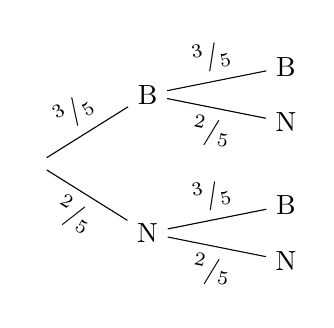
\begin{tikzpicture}[grow=right, sloped]
          % Set the overall layout of the tree
          \tikzstyle{level 1}=[level distance=4em, sibling distance=5em]
          \tikzstyle{level 2}=[level distance=5em, sibling distance=2em]
          \node {}
          child {
            node {N}
            child {
              node {N}
              edge from parent
              node[below] {$^2/_5$}
            }
            child {
              node {B}
              edge from parent
              node[above] {$^3/_5$}
            }
            edge from parent
            node[below] {$^2/_5$}
          }
          child {
            node {B}
            child {
              node {N}
              edge from parent
              node[below] {$^2/_5$}
            }
            child {
              node {B}
              edge from parent
              node[above] {$^3/_5$}
            }
            edge from parent
            node[above] {$^3/_5$}
          };
        \end{tikzpicture}
      \end{center}

      \columnbreak

      \begin{itemize}
        \item Une seule branche correspond à \og{}Obtenir deux noires\fg{}. Sa probabilité est le produit des probabilités sur son chemin. Donc $P(A)=\frac{2}{5}\times\frac{2}{5}=\frac{4}{25}$.
        \item Deux branches correspondent à \og{}Obtenir une blanche et une
          noire\fg{}. La probabilité de $B$ est la somme des probabilités de ces
          branches :
          $P(B)=\frac{2}{5}\times\frac{3}{5}+\frac{3}{5}\times\frac{2}{5}=\frac{12}{25}$.
      \end{itemize}
    \end{multicols}
\end{exemple}

